\documentclass{article}
\usepackage[utf8]{inputenc}
\title{Video 2: the standard error}
\author{wbg231 }
\date{December 2022}
\newcommand{\R}{$\mathbb{R}$}
\newcommand{\B}{$\beta$}
\newcommand{\A}{$\alpha$}
\newcommand{\D}{\Delta}

\newcommand{\avector}[2]{(#1_2,\ldots,#1_{#2})}
\newcommand{\makedef}[2]{$\textbf{#1}$:#2 }
\usepackage{tikz,graphicx,hyperref,amsmath,amsfonts,amscd,amssymb,bm,cite,epsfig,epsf,url}

\begin{document}

\maketitle

\section{introduction}
\begin{itemize}
\item \href{https://www.youtube.com/watch?v=wzWrZ40ZPoU&list=PLBEf5mJtE6KuZ5NBQMuWIMsiOOrV9ibzm&index=67}{video link}
\item continuing talking about estimating population parameters from limited data
\item today we are talking about standard error
\item typically population parameters are things that we could in principal calculate and should be constant. 
\itme we try to estimate them using a random sub set of the population a sample that we use for calculation ,this thing is a random variable that is dependant on our sample
\item often during this analysis we will talk about population mean, and sample mean because they are simple and easy to work with, but in general there are many population parameters
\section{random sampling }
\item data $a_1...a_k$
\item random samples $\Tilde{x}_1...\Tilde{x}_n$ f
\item \textbf{here i am saying there are k individuals in the population (in the slides they use N) and n individuals in the sample in the slides they use n}
\item samples are independent and identically distributed random variables with pmf $p_{\Tilde{x}_{j}}(a_i)=P(\Tilde{x}_{j}=a_i)=\frac{1}{k}$ so each individual in the population has an equal chance of being chosen. 
\item heights and sample means are tightly concentrated around the true population mean 
\item sample means has to be analyzed probabilistic ally because it is a random variable 
\subsection{sample mean }
\item $\Tilde{m}=\frac{1}{n}\Sigma_{i=1}^{n}\Tilde{x}_i$
\item $E[\Tilde{m}]=\mu_{pop}$ so in other words we know that sample mean is unbiased 
\item this alone does not make sample mean a good estimator of population mean, because we have not said anything about its variance 
\item if the estimator has high variance then there is a high probability that it will be far away from our parameter of interests are we would like 
\section{standard error}
\item for random measurements $\Tilde{x}_1...\Tilde{x}_n$
\item deterministic parameter of interests $\gamma$
\item  estimator $h(\Tilde{x}_1...\Tilde{x}_n)$ which is unbiased ie $E[h(\Tilde{x}_1...\Tilde{x}_n)]=\gamma$
\item the standard error of the estimator is the standard deviation $se[h(\Tilde{x}_1...\Tilde{x}_n)]=\sqrt{var(h(\Tilde{x}_1...\Tilde{x}_n))}$
\item this is standard error because the estimator is unbiased meaning that $E[h(\Tilde{x}_1...\Tilde{x}_n)]=\gamma$
\item meaning that $se(h(\Tilde{x}_1...\Tilde{x}_n))=\sqrt{var(h(\Tilde{x}_1...\Tilde{x}_n))}=\sqrt{E[(h(\Tilde{x}_1...\Tilde{x}_n)-E[h(\Tilde{x}_1...\Tilde{x}_n)])^2]}=\sqrt{E[(h(\Tilde{x}_1...\Tilde{x}_n)-\gamma)^2]}$ so this is the square root of mean squared error
\item so in other words the variance of an unbiased estimator can be thought of as the error ie on average how far off our estimator is from the population parameter it is estimating so in general we want it as small as possible
\subsection{standard error of the sample mean}
 \item we know sample mean is unbiased
 \item $se[\Tilde{m}]^2=var(\Tilde{m})=var(\frac{1}{n}\Sigma_{j=1}^{n}\Tilde{x}_{j})=\frac{1}{n^2}var[\Sigma_{j=1}^{N}\Tilde{x}_j]$
 \item recall that if $\Tilde{a}, \Tilde{b}$ are uncorrelated $$var(\Tilde{a}\Tilde{b})=var(a)+var(b)+2cov(a,b)=var(a)+var(b)$$
 \item thus as we know $\Tilde{x}_i\Tilde{x}_{j}$ are independent for all i and j and have finite variance we can say$se[\Tilde{m}]^2=var(\Tilde{m})=var(\frac{1}{n}\Sigma_{j=1}^{n}\Tilde{x}_{j})=\frac{1}{n^2}var[\Sigma_{j=1}^{N}\Tilde{x}_j]=\frac{1}{n^2}\Sigma_{j=1}^{n}var(\Tilde{x}_{j})$
 \item so now we want to reason about $var(\Tilde{x}_j)$ we know that $var(\Tilde{x}_j)=E[(\Tilde{x}_j-E[\Tilde{x}_j])^2]=E[(\Tilde{x}_j-\mu_{pop})^2]=\Sigma_{i=1}^{k}(a-\mu_{pop})^2P(\Tilde{x}_{j}=a_i)=\frac{1}{k}\Sigma_{i=1}^{k}(a-\mu_{pop})^2=\frac{1}{k}\Sigma_{i=1}^{k}\sigma_{pop}^2=\sigma_{pop}^2$
 \item so tun ring back to standard error we can write $se[\Tilde{m}]^2=var(\Tilde{m})=var(\frac{1}{n}\Sigma_{j=1}^{n}\Tilde{x}_{j})=\frac{1}{n^2}var[\Sigma_{j=1}^{N}\Tilde{x}_j]=\frac{1}{n^2}\Sigma_{j=1}^{n}var(\Tilde{x}_{j})=\frac{1}{n^2}\Sigma_{j=1}^{n}\sigma^2_{pop}=\frac{n\sigma^2_{pop}}{n^2}=\frac{\sigma_{pop}^2}{n}$
 \item so thus we can see that $se(\Tilde{m})=\frac{\sigma_{pop}}{\sqrt{n}}$
\item so that is the standard error is a function of the population variance and the size of our sample
\item notice that K does not matter !
\item notice further that $se(\Tilde{m})=\frac{\sigma_{pop}}{\sqrt{n}}$ is decreasing with the square root of n. 
\item this tells us how our accuracy will scale as we increase the size of our sample
\item \item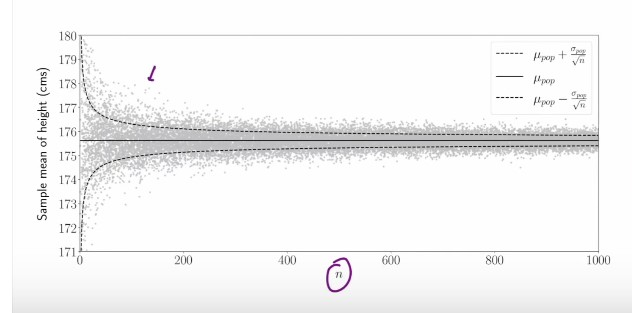
\includegraphics[width=10cm]{notes/week_3/Video 2: the standard error/immages/v_2_1.jpg}
\item this chart tells us a lot. namely that as we increase n ie our sample size  our sample average will trend towards the population average, but this is not a hard bound this is all probabilistic there are still exceptions to this, 
\item so we can see the spread decreases at $\frac{1}{\sqrt{n}}$ which is what we expected to see. 
\subsection{sample proportion}
\item covid prevalence in NYC
\item $\theta_{pop}=.05$ is our parameter of interest
\item we see that, the sample proportion changes as we take different samples, but the population proportion does not change
\item we know that sample proportion is an unbiased estimator of the population proportion
\item recall that in this setting our population is $a_1...a_k$ where $a_i=1$ if the ith person has covid and zero otherwise
\item random samples $\Tilde{x}_{1}...\Tilde{x}_{n}$ which are iid with probability mass function $P(\Tilde{x}_{i}=a_j)=\frac{1}{k}\forall i,j$
\item so recall the sample proportion in this set up is the same mean that is  $\Tilde{m}=\frac{1}{n}\Sigma_{j=1}^{n}\Tilde{x}_{j}=\frac{\text{ people with covid in sample}}{n}$ 
\item so we can then apply our previous result to see that the standard error of the sample proportion is $se[\Tilde{m}]=\frac{\sigma_{pop}}{\sqrt{n}}$ 
\item so what is $\sigma_{pop}^{2}$ in this case? $\sigma_{pop}^{2}=\frac{1}{k}\Sigma_{i=1}^{k}(a_i-\theta_{pop})^{2}$ the mean is the population proportion 
\item we can expand this and see that $\sigma_{pop}^{2}$ in this case? $\sigma_{pop}^{2}=\frac{1}{k}\Sigma_{i=1}^{k}(a_i-\theta_{pop})^{2}=\frac{1}{K}\Sigma_{i=1}^{k}a_i^2-\frac{2\theta_{pop}}{K}\Sigma_{i=1}^{k}a_i+\frac{1}{K}\Sigma_{i=1}^{k}\theta_{pop}^2=\frac{1}{K}\Sigma_{i=1}^{k}a_i^2-{2\theta_{pop}^2}+{\theta_{pop}^2}$ as we know $a_i=0 \text{ or} a_i=1$ only $a_i^2=a_i$ and thus $\frac{1}{K}\Sigma_{i=1}^{k}a_i^2-{2\theta_{pop}^2}+{\theta_{pop}^2}=\frac{1}{K}\Sigma_{i=1}^{k}a_i-{2\theta_{pop}^2}+{\theta_{pop}^2}={\theta_{pop}}-{\theta_{pop}^2}=
(\theta_{pop})(1-\theta_{pop})$ this is pretty much the variance of a Bernoulli parameter 
\item so we can go back and plug that in and see that the standard error of the sample proportion is 
$se[\Tilde{m}]=\frac{\sigma_{pop}}{\sqrt{n}}=\sqrt{\frac{(\theta_{pop})(1-\theta_{pop})}{n}}$ 
\item we further know that $(\theta_{pop})(1-\theta_{pop})\in [0,1]$ so thus $se[\Tilde{m}]=\frac{\sigma_{pop}}{\sqrt{n}}=\sqrt{\frac{(\theta_{pop})(1-\theta_{pop})}{n}}$  will scale with $\frac{1}{\sqrt{n}}$
\item then we go through a numeric example which more or less shows that the spread of our sample proportion falls by $\frac{1}{\sqrt{n}}$ like we expected
\item so the take away of this is random sampling will allow an unbiased estimator to approximate a population parameter well, due to the fact that the estimator is unbiased, and the standard error will fall as a function of the sample size. 

\end{itemize}
\end{document}
